\documentclass{article}

\usepackage{graphicx}
\usepackage{amsmath}
\usepackage{amsthm}
\usepackage{amssymb}
\usepackage{url}
\usepackage{multirow}
\usepackage{times}
\usepackage{fullpage}
\usepackage{listings}

\newcommand{\comment}[1]{}

\title{CS315: Group G03 \\
Database system with temporal Warehousing\\
{\bf Medicate} }
\author{
\begin{tabular}{ccc}
	Prashant Jalan & S Sai Krishna Prasad & Soniya Barmate \\
	11523 (18) & 11620 (17) & 11725 (63) \\
	\url{prasant@iitk.ac.in} & \url{ssai@iitk.ac.in} & \url{barmate@iitk.ac.in} \\
	\multicolumn{3}{c}{Dept. of Computer Science \& Engineering, IITK}
\end{tabular}
}
\date{Report \\	% replace by ``initial'' or ``final'' as appropriate
12th April, 2014}	% replace by actual date of submission or \today

\begin{document}

\maketitle

\begin{abstract}
	%
	Time plays a very important role in information systems. Every institution have the problem of its data becoming out of date but which is valuable in decision making process.A Temporal database is a database which has built-in support for handling data involving time and helps us in analysing historical trends through which we can infer the decision making process. Temporal warehousing helps us to provide a systematic way of dealing with the data involving time. In this work, we try to built an online portal to maintain online medical records, in which the patient/doctor can query data items in a temporal manner.
	%
\end{abstract}

\section{Introduction and Problem Statement}

A Data Warehouse is an architectual structure that supports the management of $``$Subject-oriented$"$, $``$Integrated$"$, $``$Time-variant$"$ and $``$Non-volatile$"$ data. A Temporal Database is inroduced as a database that supports $``$Valid time$"$ (i.e. the time when the fact becomes effective in reality), or $``$Transaction time$"$ (i.e. the time when the fact is stored in the database), or both times.

\subsection{Related Material}

{\bf Flask}\cite{bib2} is a lightweight web based application framework which is written in python and based on the Werkzeug WSGI toolkit and Jinja2 template engine. We have used it to manage all the web based work which basically involves client side operations like managing cookies and data processing. 
\\\\
{\bf Python}\cite{bib3} is used to operate on the server side by connecting to the database and developing the query commands as per the requirements. The database system implementing SQL in our project is {\bf Sqlite3}\cite{bib1}. It is arelational database management system. It automatically handles concurrency, indexing, sorting, and the queries for inserting, deleting or updating the data along with various other uses.
\\\\
We have collected the database of diseases, its symptoms and the drugs required from the website \cite{bib4}.

\newpage
\section{Algorithm or Approach}

The following are the five major categories of tables that we have used in the database:-

\begin{enumerate}
\item Doctor: It stores the details of the doctor including his name, address, contact number, email id and password. The table is in BCNF (taking contact number and place as an single entity). We have used indexing in the the doctors email id. The indexing is used for optimising the query time for the queries performed during login session.
\item Patient: It stores the details of the patient including his name, address, contact number, email id, password, date of birth and blood group. The table is in BCNF (taking contact number and place as an single entity). We have used indexing in the the patients email id. The indexing is used for optimising the query time for the queries performed during login session.
\item A table for each year for storing the patient records of that year. Each table stores the details of the illness the patient suffered from, in that particular year includng the date, type of illness, the email id of the patient, the email id of the doctor who diagnosed him, and a unique id created for referencing to other tables. This table is in BCNF. We have used indexing for the following fields:
\begin{itemize} 
\item Email id of doctor: For optimising the queries when the patient records diagonised by a particular doctor needs to be pulled up.
\item Email id of patient: For optimising the queries when a patient wants to see his past records.
\item The date on which it was diagnised: For optimising queries pulled up for particular dates.
\item Name of the disease: For optimising queries querying the most popular or least popular diseases.
\end{itemize}
\item A table for each year to store the symptoms that were shown in reference to a particular patient record. The table is in 3NF. We used indexing on the id field in ascending order which optimises the queries querying the symptoms for a particular patient record.
\item A table for each year to store the drugs that were prescribed in reference to a particular patient record. The table is in 3NF. We used indexing on the id field in ascending order which optimises the queries querying the symptoms for a particular patient record.
\end{enumerate}

We populated the tables with randome entries for testing. Please note that our system is {\bf scalable} because as the number of entries in a particular table increases we can have a different time based table. For instance, now we have new tables every year, but in case of more traffic we can have new tables every six months. Currently, number of entries are:
\begin{itemize}
\item Patient with 1 lakh entries.
\item Doctor with 1000 entries.
\item PatientRecord for each year with nearly 1 million entries. PatientSymptoms and PatientDrugs with nearly 2 million entries.
\end{itemize}

\subsection{Part of Code for Database Creation}

\begin{lstlisting}
import sqlite3

conn = sqlite3.connect('Database.db')

c = conn.cursor()

# Create table
c.execute('''CREATE TABLE if not exists doctor(name text, email text, 
password text, specialization text, contact_no int, PRIMARY KEY (email))''')
c.execute('''CREATE INDEX d_email ON doctor(email ASC)''')

c.execute('''CREATE TABLE if not exists patient(name text, email text, 
password text, DOB date, address text, contact_no int, blood_group text, PRIMARY KEY(email))''')
c.execute('''CREATE INDEX p_email ON patient(email ASC)''')

c.execute('''CREATE TABLE if not exists patientRecord2014(id int, email text,
 doc_email text, disease text, date date, PRIMARY KEY(id))''')
c.execute('''CREATE INDEX d_email_record2014 ON patientRecord2014(doc_email ASC)''')
c.execute('''CREATE INDEX p_email_record2014 ON patientRecord2014(email ASC)''')
c.execute('''CREATE INDEX date2014 ON patientRecord2014(date ASC)''')
c.execute('''CREATE INDEX disease2014 ON patientRecord2014(disease ASC)''')

c.execute('''CREATE TABLE if not exists patientSymptom2014(id int, symptom text,
 FOREIGN KEY(id) REFERENCES patientRecord2014(id))''')
c.execute('''CREATE INDEX id_symptom2014 ON patientSymptom2014(id ASC)''')

c.execute('''CREATE TABLE if not exists patientDrugs2014(id int, drugs text,
 FOREIGN KEY(id) REFERENCES patientRecord2014(id))''')
c.execute('''CREATE INDEX id_drugs2014 ON patientDrugs2014(id ASC)''')

# Save (commit) the changes
conn.commit()
conn.close()
\end{lstlisting}
\vspace{0.4in}
\subsection{Indexing and Query time}
\vspace{0.1in}
We have used the indexing on tables containing only one attribute as it optimises the result even when the attributes are `or' connected rather than `\&' connected\cite{bib5}. For example in the query\\\\{\it select * from patientRecord2012 where email = "email@patient800"}\\\\
The Explain command shows that indexing has been used\\
{\it Explain query plan select * from patientRecord2012 where email = "email@patient800"}
\begin{lstlisting}
0|0|0|SEARCH TABLE patientRecord2012 USING INDEX p\_ email\_ record2012 (email=?) (~10 rows)
0|0|0|SCAN TABLE patientRecord2012 (~100000 rows)
\end{lstlisting}

Time taken with indexing = 0.004 seconds. The time taken without indexing = 0.008 seconds\\\\
So clearly we can see that the time taken has reduced by half with indexing and the scaning of rows has reduced to 10 rows from 100000 rows.\\\\{\bf Similarly, we optimised the various queries we wrote at the server side}.

\newpage
\section{Results}

We designed a fully working Python based web server which provides on the client side an online portal with login/logout facility, facility to add past medical records and perform diffent query operations. The code can be found out at \cite{bib7}.
Fig:\ref{PR} and Fig:\ref{DR} shows the screenshots for patient registration and doctor registration respectively. Fig:\ref{entry} shows the screenshot for inserting a medical entry.\\\\

\begin{figure}[!htbp]
	\centering
	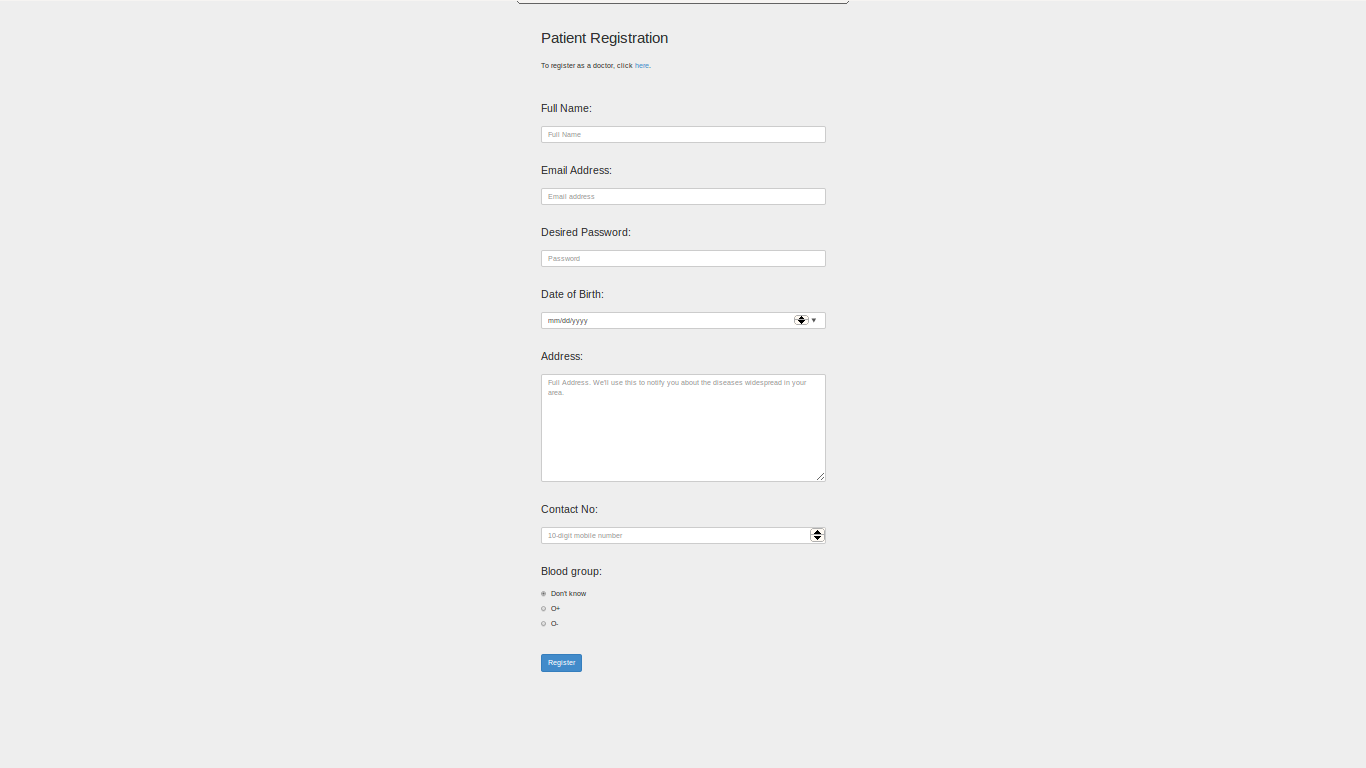
\includegraphics[width=0.8\columnwidth]{patient_reg.png}
	\caption{Patient Registration}
	\label{PR}
\end{figure}

\begin{figure}[!htbp]
	\centering
	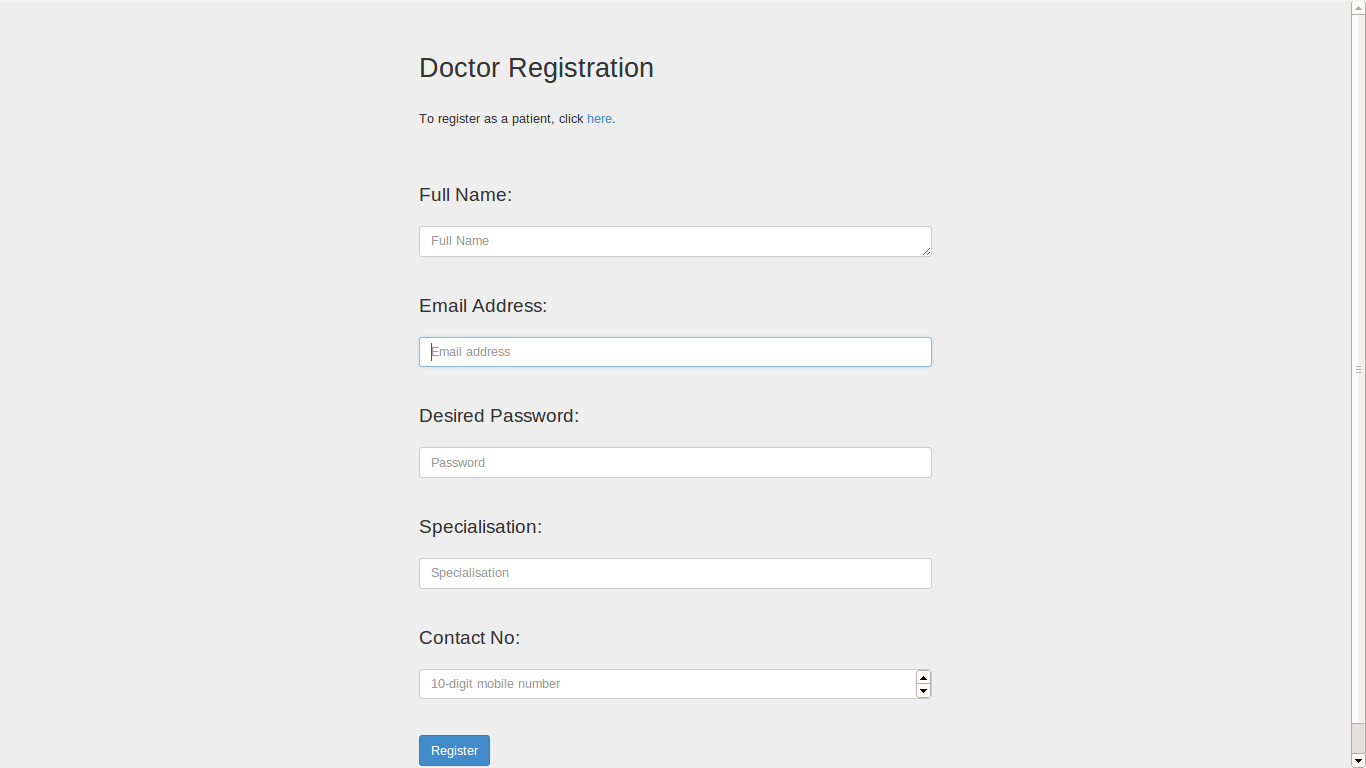
\includegraphics[width=0.8\columnwidth]{doctor_reg.png}
	\caption{Doctor Registration}
	\label{DR}
\end{figure}

\begin{figure}[!htbp]
	\centering
	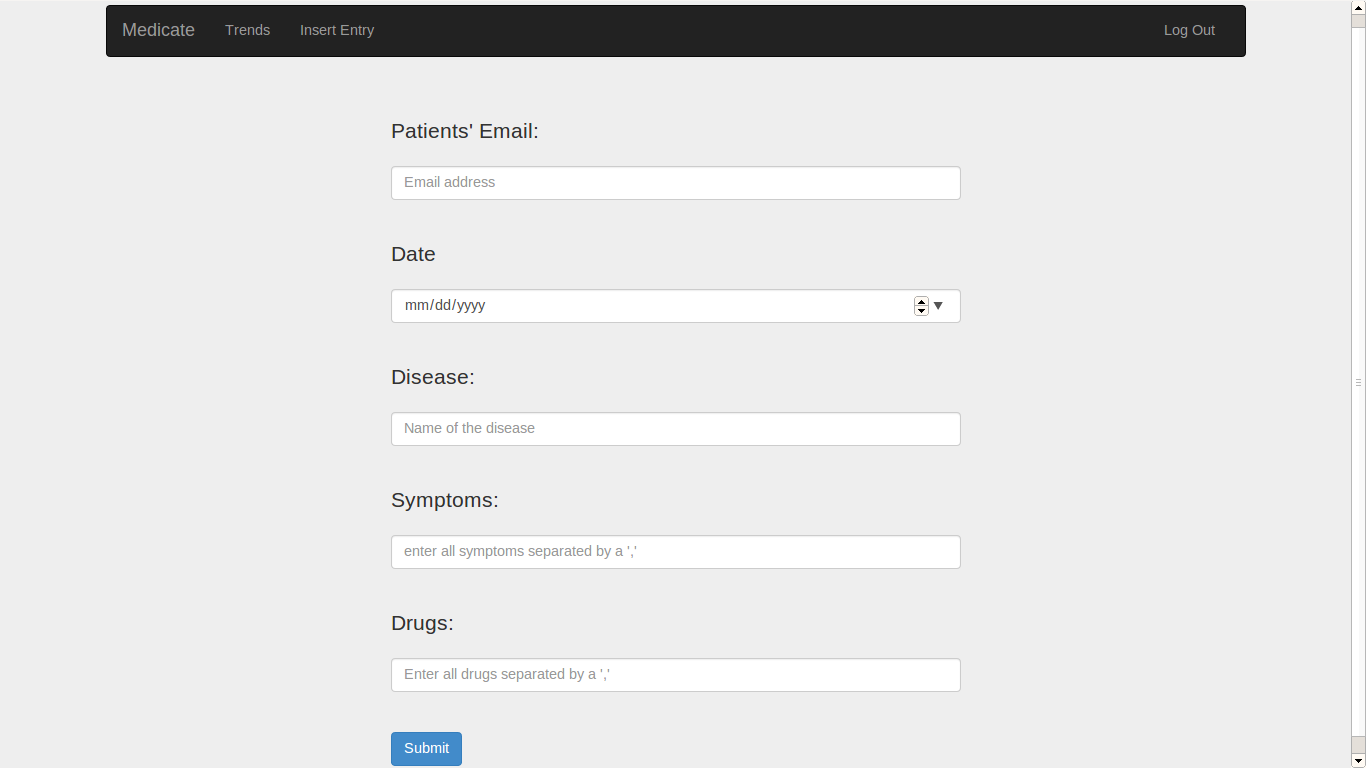
\includegraphics[width=0.8\columnwidth]{entry.png}
	\caption{Inserting New Entry}
	\label{entry}
\end{figure}

\newpage
We are able to query these kind of queries:
\begin{itemize}
\item How many people were having any particular disease at a particular time?\\\\
\textit{select * from patientRecord2013 where disease = "diseasename" and date between '2013-01-01' and '2013-05-06';}
\item How many people are having disease on a particular day?\\\\
\textit{select * from patientRecord2013 where date between '2013-01-01' and '2013-05-06';}
\item What kind of symptoms are being discovered for a particular disease?
\item How is the trend of a disease change with respect to time?
\item What is the most popular disease at a time range for each year?
\item How the records of a doctor are changing with respect to the years?
\item Historic trends of the diseases of a patient.
\end{itemize}

\section{Conclusions}

We can use it as an online prescription form.It can be used to predict diseases from the given symptoms using machine learning techniques and we can also try to subscribe medicines to patients who cant buy costly medicines by looking at the constituents of the prescribed medicines.Significantly fewer errors found within personal health records.Faster care and decision making responses from assigned medical professionals.

\newpage
\begin{thebibliography}{9}


\bibitem{bib1} 
Sqlite3. \url{http://www.sqlite.org/docs.html}

\bibitem{bib2}
Flask. \url{http://flask.pocoo.org/docs/}

\bibitem{bib3}
Python 2.7 \url{https://docs.python.org/2/}

\bibitem{bib4} 
Most common diseases, their symptoms and cure. \url{http://www.ranker.com/}.

\bibitem{bib5}
Query Planner. \url{http://sqlite.org/queryplanner.html}

\bibitem{bib7}
Code for Medicate. \url{https://github.com/PrashantJalan/Medicate}

\end{thebibliography}
\end{document}